\section{Related Work}
\label{sec:related}

This section provides a quick overview of the security concepts needed to
analyze Intel's SGX, and describes the broader picture of trusted hardware
projects that SGX belongs to. Table~\ref{fig:secure_processors} summarizes the
security properties of SGX and the other trusted hardware presented here.

\begin{table*}
  \centering
  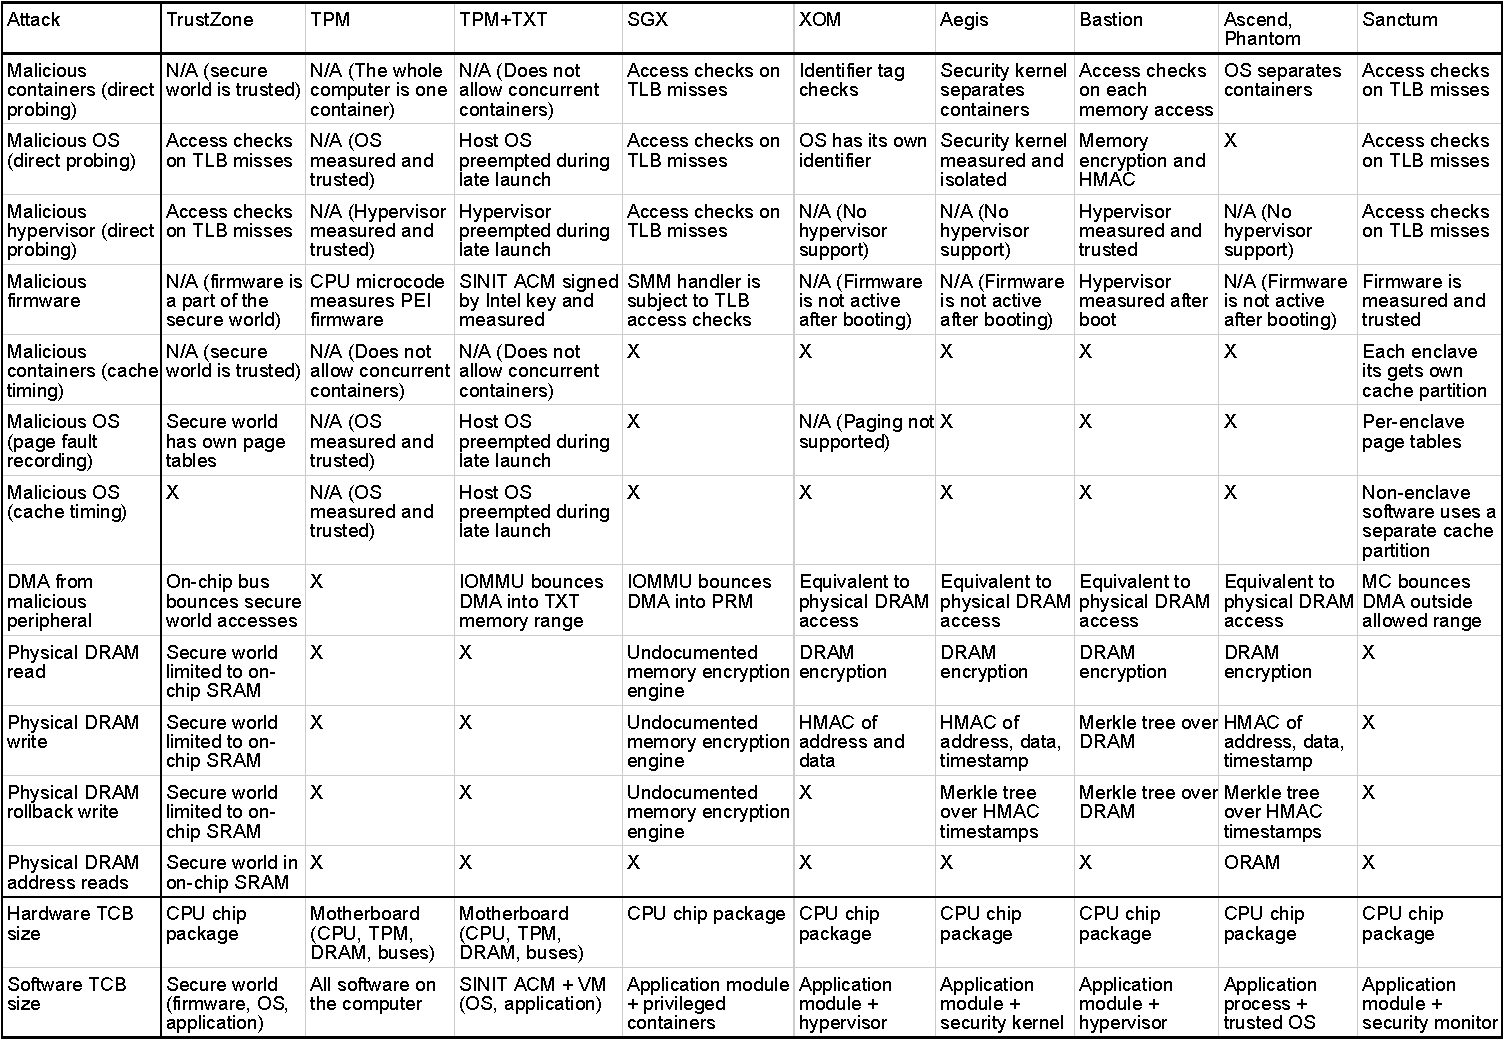
\includegraphics[angle=90,width=170mm]{figures/secure_processors_table.pdf}
  \caption{
    Security features overview for the trusted hardware projects related to
    Intel's SGX
  }
  \label{fig:secure_processors}
\end{table*}


\section{Security Model}
\label{sec:attestation}

THe central context of SGX is the \textit{enclave}, a protected environment
that contains the code and data pertaining to a security-sensitive computation.
An SGX-enabled processor protects the integrity and privacy of the computation
inside an enclave by isolating the enclave's code and data from the outside
environment, including the operating system and hypervisor, and hardware
devices attached to the system bus. At the same time, the SGX model remains
compatible with the the traditional software layering in the Intel
architecture, where the OS kernel and hypervisor manage the computer's
resources. The rest of this section describes the security properties of
enclaves, discussing the trade-offs made while trying to balance security with
backwards compatibility.



Enclaves were designed to contain and protect the privacy-sensitive parts of an
application. All the code that handles private data must receive integrity
protection. Otherwise, a hostile environment could modify the code to leak
information about private data. Therefore, the SGX programming model prescribes
that code which accesses private data must be entirely contained inside an
enclave. Jumping into and out of enclave code must be performed explicitly
using the dedicated instructions \texttt{EENTER} and \texttt{EEXIT}.

The code inside an enclave runs at ring 3 (user mode), so it has the same
privileges as regular application code (see Figure \ref{fig:cpu_rings}).

\begin{figure}[hbtp]
  \center{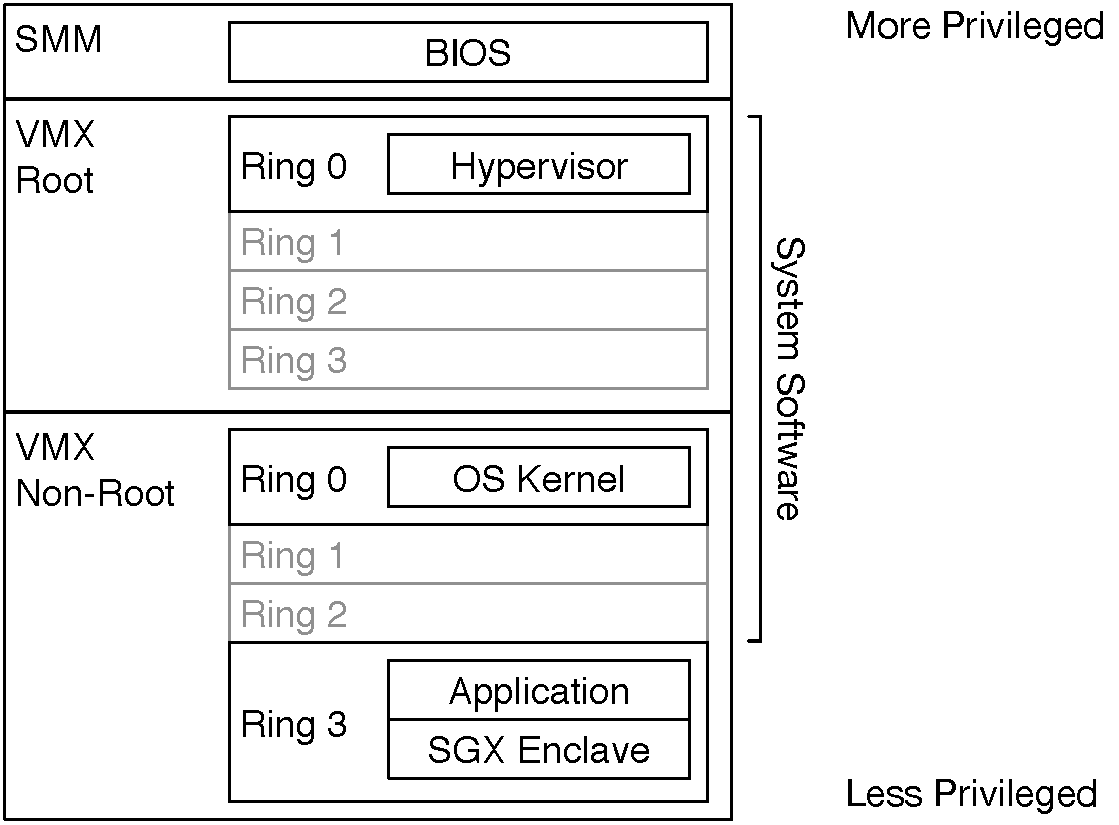
\includegraphics[width=75mm]{figures/cpu_rings.pdf}}
  \caption{
    Enclaves hold an application's private data and the code that operates on
    it. Therefore, they run at ring 3, in user mode.
  }
  \label{fig:computing_model}
\end{figure}

\HeadingLevelB{Cache Timing Attacks}
\label{sec:cache_timing}

Cache timing attacks~\cite{banescu2011cache} are a powerful class of software
attacks that can be mounted entirely by application code running at ring 3
(\S~\ref{sec:rings}). Cache timing attacks do not learn information by reading
the victim's memory, so they bypass the address translation-based isolation
measures (\S~\ref{sec:paging}) implemented in today's kernels and hypervisors.


\HeadingLevelC{Theory}

Cache timing attacks exploit the unfortunate dependency between the location of
a memory access and the time it takes to perform the access. A cache miss
requires at least one memory access to the next level cache, and might require
a second memory access if a write-back occurs. On the Intel architecture, the
latency between a cache hit and a miss can be easily measured by the
\texttt{RDTSC} and \texttt{RDTSCP} instructions (\S~\ref{sec:address_spaces}),
which read a high-resolution time-stamp counter. These instructions have been
designed for benchmarking and optimizing software, so they are available to
ring 3 software.

The fundamental tool of a cache timing attack is an attacker process that
measures the latency of accesses to carefully designated memory locations in
its own address space. The memory locations are chosen so that they map to
the same cache lines as some interesting memory locations in a victim process,
in a cache that is shared between the attacker and the victim. This requires
in-depth knowledge of the shared cache's organization (\S~\ref{sec:cache_org}).

Armed with the knowledge of the cache's organization, the attacker process
sets up the attack by accessing its own memory in such a way that it fills up
all the ways in the cache sets that would hold the victim's interesting memory
locations. After the targeted cache sets are full, the attacker allows the
victim process to execute. When the victim process accesses an interesting
memory locations in its own address space, the shared cache must evict one of
the cache lines holding the attacker's memory locations.

As the victim is executing, the attacker process repeatedly times accesses to
its own memory locations. When the access times indicate that a location was
evicted from the cache, the attacker can conclude that the victim accessed an
interesting memory location in its own cache. Over time, the attacker collects
the results of many measurements and learns a subset of the victim's memory
access pattern. If the victim processes sensitive information using
data-dependent memory fetches, the attacker may be able to deduce the sensitive
information from the learned memory access pattern.


\HeadingLevelC{Practical Considerations}

Cache timing attacks require control over a software process that shares a
cache memory with the victim process. Therefore, a cache timing attack that
aims at the L2 cache would have to rely on the system software to schedule a
software thread on a logical processor in the same core as the target software,
whereas an attack on the L3 cache can be performed using any logical processor
on the same CPU. The latter attacks rely on the fact that the L3 cache is
inclusive, which greatly simplifies the processor's cache coherence
implementation (\S~\ref{sec:cache_coherence}).

The cache sharing requirement implies that L3 cache attacks are feasible in an
IaaS environment, whereas L2 cache attacks become a significant concern when
running sensitive software on a user's desktop.

Out-of-order execution (\S~\ref{sec:out_of_order}) can introduce noise in cache
timing attacks. First, memory accesses may not be performed in program order,
which can impact the lines selected by the cache eviction algorithms. Second,
out-of-order execution may result in cache fills that do not correspond to
executed instructions. For example, a load that follows a faulting instruction
may be scheduled and executed before the fault is detected.

Cache timing attacks must account for speculative execution, as mispredicted
memory accesses can still cause cache fills. Therefore, the attacker may
observe cache fills that don't correspond to instructions that were actually
executed by the victim software. Memory prefetching adds further noise to cache
timing attacks, as the attacker may observe cache fills that don't correspond
to instructions in the victim code, even when accounting for speculative
execution.


\HeadingLevelC{Known Cache Timing Attacks}

Despite these difficulties, cache timing attacks are known to retrieve
cryptographic keys used by AES~\cite{osvik2006aes, bonneau2006aes},
RSA~\cite{brumley2005rsa}, Diffie-Hellman~\cite{kocher1996timing}, and
elliptic-curve cryptography~\cite{brumley2011ecc}.

Early attacks required access to the victim's CPU core, but more sophisticated
recent attacks~\cite{yarom2013llctiming, liu2015llctiming} are able to use the
L3 cache, which is shared by all the cores on a CPU die. L3-based attacks can
be particularly devastating in cloud computing scenarios, where running
software on the same computer as a victim application only requires modest
statistical analysis skills and a small amount of
money~\cite{ristenpart2009colocation}. Furthermore, cache timing attacks were
recently demonstrated using JavaScript code in a page visited by a Web
browser~\cite{oren2015jstiming}.

Given this pattern of vulnerabilities, ignoring cache timing attacks is
dangerously similar to ignoring the string of demonstrated attacks which led to
the deprecation of SHA-1~\cite{nist2014sha1policy, google2014sha1deprecation,
microsoft2014sha1deprecation}.


\HeadingLevelC{Defending against Cache Timing Attacks}
\label{sec:cache_timing_workarounds}

Fortunately, invalidating any of the preconditions for cache timing attacks is
sufficient for defending against them. The easiest precondition to focus on is
that the attacker must have access to memory locations that map to the same
sets in a cache as the victim's memory. This assumption can be invalidated by
the judicious use of a cache partitioning scheme.

Performance concerns aside, the main difficulty associated with cache
partitioning schemes is that they must be implemented by a trusted party. When
the system software is trusted, it can (for example) use the principles behind
page coloring~\cite{taylor1990coloring, kessler1992coloring} to partition the
caches~\cite{lin2008coloring} between mutually distrusting parties. This comes
down setting up the page tables in such a way that no two mutually distrusting
software module are stored in physical pages that map to the same sets in any
cache memory.  However, if the system software is not trusted, the cache
partitioning scheme must be implemented in hardware.

The other interesting precondition is that the victim must access its memory in
a data-dependent fashion that allows the attacker to infer private information
from the observed memory access pattern. It becomes tempting to think that
cache timing attacks can be prevented by eliminating data-dependent memory
accesses from all the code handling sensitive data.

However, removing data-dependent memory accesses is difficult to accomplish in
practice because instruction fetches must also be taken into consideration.
\cite{kasper2009aes} gives an idea of the level of effort required for removing
data-dependent accesses from AES, which is a relatively simple data processing
algorithm. At the time of this writing, we are not aware of any approach that
scales to large pieces of software.

While the focus of this section is cache timing attacks, we would like to point
out that any shared resource can lead to information leakage. A worrying
example is hyper-threading (\S~\ref{sec:cpu_core}), where each CPU core is
represented as two logical processors, and the threads executing on these two
processors share execution units. An attacker that can run a process on a
logical processor sharing a core with a victim process can use
\texttt{RDTSCP}~\cite{petters1999making} to learn which execution units are in
use, and infer what instructions are executed by the victim process.

\subsection{The IBM 4765 Secure Coprocessor}

Secure coprocessors~\cite{yee1994coprocessors} encapsulate an entire computer
system, including a CPU, a cryptographic accelerator, caches, DRAM, and an I/O
controller within a tamper-resistant environment. The enclosure includes
hardware that deters attacks, such as a Faraday cage, as well as an array of
sensors that can detect tampering attempts. The secure coprocessor destroys the
secrets that it stores when an attack is detected. This approach has good
security properties against physical attacks, but tamper-resistant enclosures
are very expensive~\cite{anderson2001security}, relatively to the cost of a
computer system.

The IBM 4758~\cite{smith1999ibm4758}, and its most current-day successor, the
IBM 4765~\cite{nist2015ibm4765} (shown in Figure~\ref{fig:ibm_4765}) are
representative examples of secure coprocessors. The 4758 was certified to
withstand physical attacks to FIPS 140-1 Level 4~\cite{smith1999validating},
and the 4765 meets the rigors of FIPS 140-2 Level 4~\cite{nist2011fipscert}.

\begin{figure}[hbt]
  \centering
  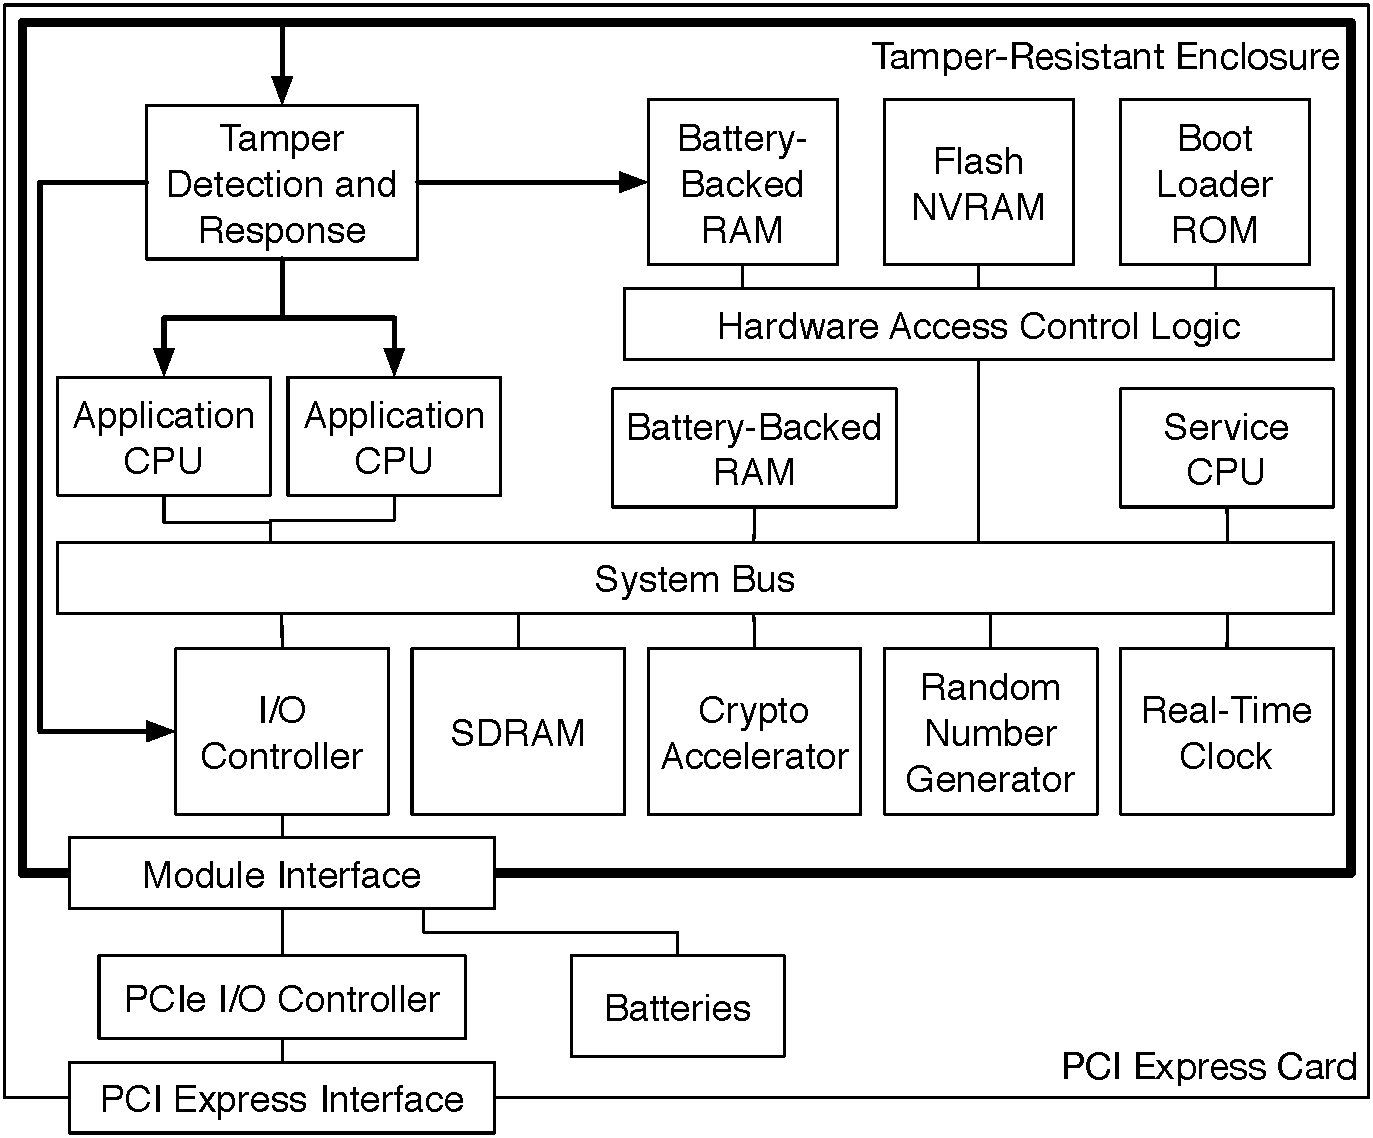
\includegraphics[width=85mm]{figures/ibm_4765.pdf}
  \caption{
    The IBM 4765 secure coprocessor consists of an entire computer system
    placed inside an enclosure that can deter and detect physical attacks.
    The application and the system use separate processors. Sensitive memory
    can only be accessed by the system code, thanks to access control checks
    implemented in the system bus' hardware. Dedicated hardware is used to clear
    the platform's secrets and shut down the system when a physical attack is
    detected.
  }
  \label{fig:ibm_4765}
\end{figure}

The 4765 relies heavily on physical isolation for its security properties. Its
system software is protected from attacks by the application software by
virtue of using a dedicated service processor that is completely separate from
the application processor. Special-purpose bus logic prevents the application
processor from accessing privileged resources, such as the battery-backed
memory that stores the system software's secrets.

The 4765 implements software attestation. The coprocessor's attestation key is
stored in battery-backed memory that is only accessible by the service
processor. Upon reset, the service processor executes a first-stage bootloader
stored in ROM, which measures and loads the system software. In turn, the
system software measures the application code stored in NVRAM and loads it into
the DRAM chip accessible to the application processor. The system software
provides attestation services to the application loaded inside the coprocessor.

\subsection{ARM TrustZone}

ARM's TrustZone~\cite{alves2004trustzone} is a collection of hardware modules
that can be used to conceptually partition a system's resources between a
\textit{secure world}, which hosts a secure container, and a \textit{normal
world}, which runs an untrusted software stack. The TrustZone
documentation~\cite{arm2009trustzone} describes semiconductor intellectual
property cores (IP blocks) and ways in which they can be combined to achieve
certain security properties, reflecting the fact that ARM is an IP core
provider, not a chip manufacturer. Therefore, the mere presence of TrustZone IP
blocks in a system is not sufficient to determine whether the system is secure
under a specific threat model. Figure~\ref{fig:trustzone} illustrates a design
for a smartphone \textit{System-on-Chip} (SoC) design that uses TrustZone IP
blocks.

\begin{figure}[hbt]
  \centering
  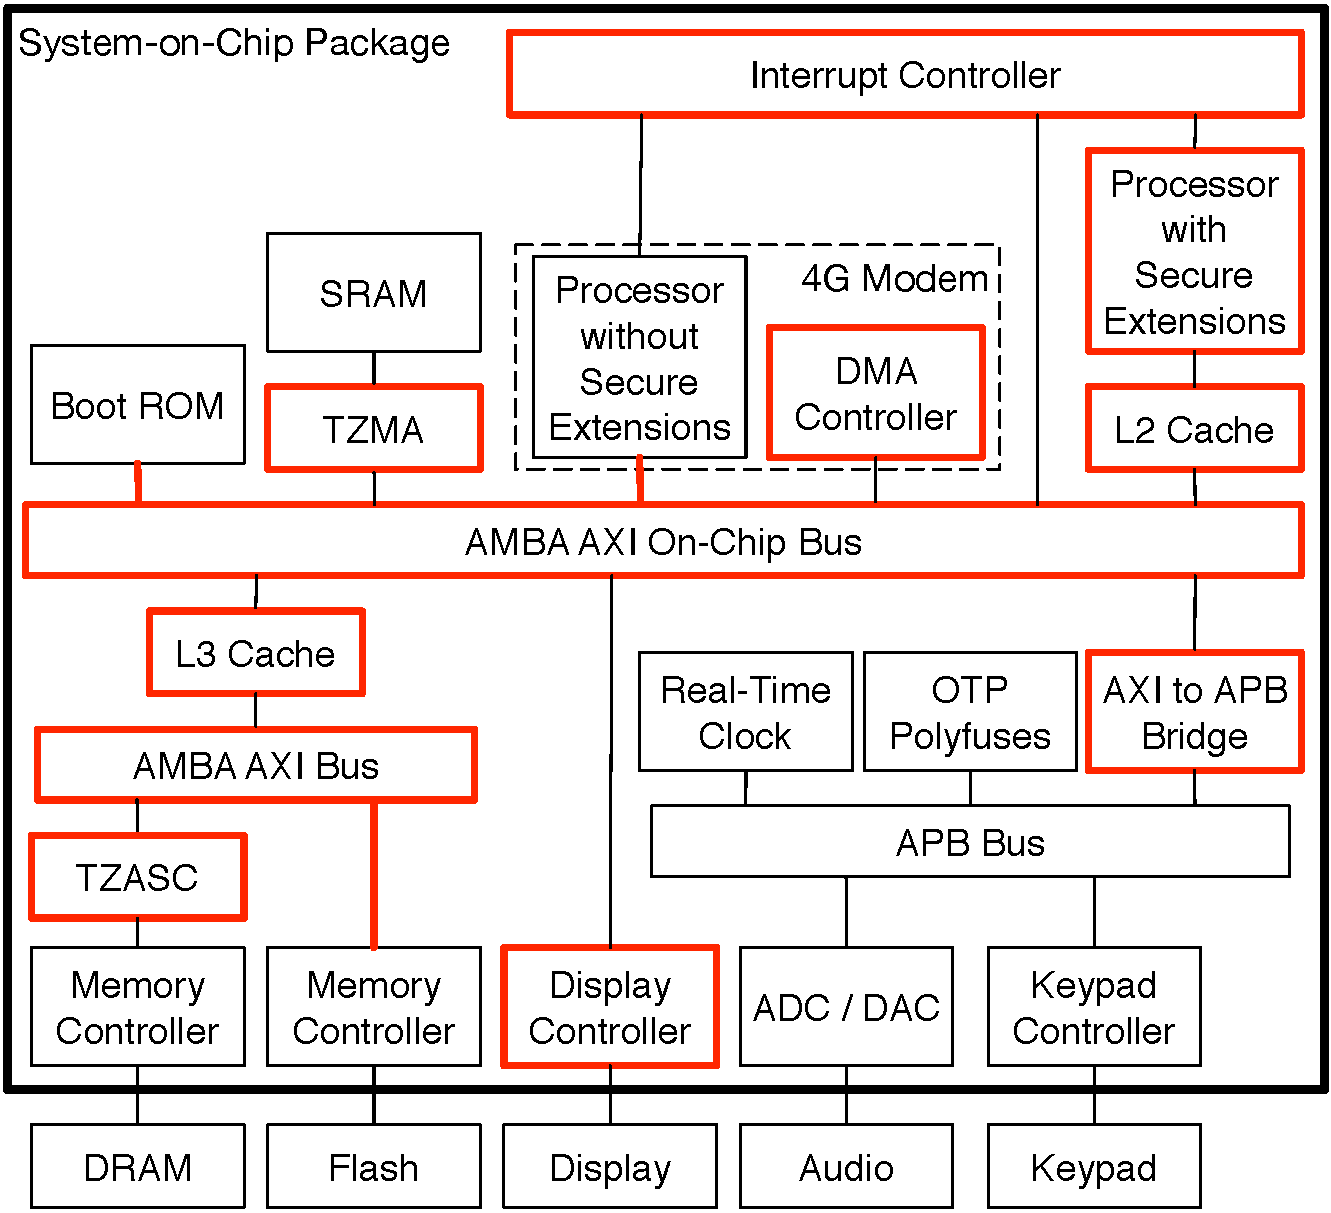
\includegraphics[width=85mm]{figures/trustzone.pdf}
  \caption{
    Smart SoC design based on TrustZone. The red IP blocks are TrustZone-aware.
    The red connections ignore the TrustZone secure bit in the bus address.
    Defining the system's security properties requires a complete understanding
    of all the red elements in this figure.
  }
  \label{fig:trustzone}
\end{figure}

TrustZone extends the address lines in the AMBA AXI system
bus~\cite{arm2004ambaxi} with one signal that indicates whether an access
belongs to the secure or normal (non-secure) world. ARM processor cores that
include TrustZone's ``Security Extensions'' can switch between executing code
in the normal world and code in the secure world. The address in each bus
access executed by a core reflects the world that the core is currently
executed.

The reset circuitry in a TrustZone processor places it in secure mode, and
points it to the first-stage bootloader stored in on-chip ROM. TrustZone's TCB
includes this bootloader, which initializes the platform, sets up the TrustZone
hardware to protect the secure container from untrusted software, and loads the
normal world's bootloader. The secure container must also implement a monitor
that performs the context switches needed to transition an execution core
between the two worlds. The monitor must also handle hardware exceptions, such
as interrupts, and route them to the appropriate world.

The TrustZone design gives the secure world's monitor unrestricted acces to the
normal world, so the monitor can implement inter-process communication (IPC)
between the software in the two worlds. Specifically, the monitor can issue
bus accesses using both secure and non-secure addresses. In general, the secure
world's software can compromise any level in the normal world's software stack.
For example, the secure container's software can jump into arbitrary locations
in the normal world by flipping a bit in a register. The untrusted software in
the normal world can only access the secure world via an instruction that jumps
into a well-defined location inside the monitor.

Conceptually, each TrustZone CPU core provides separate address translation
units for the secure and normal worlds. This is implemented by two page table
base registers, and by having the page walker use the page table base
corresponding to the core's current world. The physical addresses in the page
table entries are extended to include the values of the secure bit to be issued
on the AXI bus. The secure world is protected from untrusted software by having
the CPU core force the secure bit in the address translation result to zero for
normal world address translations. As the secure container manages its own page
tables, its memory accesses cannot be directly observed by the untrusted OS's
page fault handler.

TrustZone-aware hardware modules, such as caches, are trusted to use the secure
address bit in each bus access enforce the isolation between worlds. For
example, TrustZone's caches store the secure bit in the address tag for each
cache line, which effectively provides completely different views of the memory
space to the software running in different worlds. This design assumes that
memory space is partitioned between the two worlds, so no aliasing can occur.

The hardware modules that do not consume TrustZone's address bit are expected
to be connected to the AXI bus via IP cores that implement simple
partitioning techniques. For example, the TrustZone Memory Adapter (TZMA) can
be used to partition an on-chip ROM or SRAM into a secure region and a normal
region, and the TrustZone Address Space Controller (TZASC) partitions the
memory space provided by a DRAM controller into secure and normal regions. A
TrustZone-aware DMA controller rejects DMA transfers from the normal world that
reference secure world addresses.

It follows that analyzing the security properties of a TrustZone system
requires a precise understanding of the behavior and configuration of all the
hardware modules that are attached to the AXI bus. For example, the caches
described in TrustZone's documentation do not enforce a complete separation
between worlds, as they allow a world's memory accesses to evict the other
world's cache lines. This exposes the secure container software to cache timing
attacks from the untrusted software in the normal world. Unfortunately,
hardware manufacturers that license the TrustZone IP cores are reluctant to
disclose all the details of their designs, making it impossible for security
researchers to reason about TrustZone-based hardware.

The TrustZone components do not have any counter-measures for physical attacks.
However, a system that follows the recommendations in the TrustZone
documentation will not be exposed to physical attacks, under a threat model
that trusts the processor chip package. The AXI bus is designed to connect
components in a SoC design, so it cannot be tapped by an attacker. The
TrustZone documentation recommends having all the code and data in the secure
world stored in on-chip SRAM, which is not subjected to physical attacks.
However, this approach places significant limits on the secure container's
functionality, because on-chip SRAM is many orders of magnitude more expensive
than a DRAM chip of the same capacity.

TrustZone's documentation does not describe any software attestation
implementation. However, it does outline a method for implementing secure boot,
which comes down to having the first-stage bootloader verify a signature in the
second-stage bootloader against a public key whose cryptographic hash is burned
into on-chip \textit{One-Time Programmable} (OTP) polysilicon fuses. A hardware
measurement root can be built on top of the same components, by storing a
per-chip attestation key in the polyfuses, and having the first-stage
bootloader measure the second-stage bootloader and store its hash in an on-chip
SRAM region allocated to the secure world. The polyfuses would be gated by a
TZMA IP block that only makes them accessible to the secure world.

\HeadingLevelB{The XOM Architecture}

The execute-only memory (XOM) architecture \cite{lie2000xom} introduced the
approach of executing sensitive code and data in isolated containers managed by
untrusted host software. XOM outlined the mechanisms needed to isolate a
container's data from its untrusted software environment, such as saving the
register state to a protected memory area before servicing an interrupt.

XOM supports multiple containers by tagging every cache line with the
identifier of the container owning it, and ensures isolation by disallowing
memory accesses to cache lines that don't match the current container's
identifier. The operating system and the untrusted applications are considered
to belong to a container with a null identifier.

XOM also introduced the integration of encryption and HMAC functionality in
the processor's memory controller to protect container memory from physical
attacks on DRAM. The encryption and HMAC functionality is used for all cache
line evictions and fetches, and the ECC bits in DRAM chips are repurposed to
store HMAC values.

XOM's design cannot guarantee DRAM freshness, so the software in its containers
is vulnerable to physical replay attacks. Furthermore, XOM does not protect a
container's memory access patterns, meaning that any piece of malicious
software can perform cache timing attacks against the software in a container.
Last, XOM containers are destroyed when they encounter hardware exceptions,
such as page faults, so XOM does not support paging.

XOM predates the attestation scheme described above, and relies on a modified
software distribution scheme instead. Each container's contents are encrypted
with a symmetric key, which also serves as the container's identity. The
symmetric key, in turn, is encrypted with the public key of each CPU that is
trusted to run the container. A container's author can be assured that the
container is running on trusted software by embedding a secret into the
encrypted container data, and using it to authenticate the container. While
conceptually simpler than software attestation, this scheme does not allow the
container author to vet the container's software environment.

\HeadingLevelB{The Trusted Platform Module (TPM)}
\label{sec:sgx_related_tpm}

The Trusted Platform Module (TPM) \cite{grawrock2003tpm} introduced the
software attestation model described at the beginning of this section. The TPM
design does not require any hardware modifications to the CPU, and instead
relies on an auxiliary tamper-resistant chip. The TPM chip is only used to
store the attestation key and to perform software attestation. The TPM was
widely deployed on commodity computers, because it does not rely on CPU
modifications. Unfortunately, the cost of this approach is that the TPM has
very weak security guarantees, as explained below.

The TPM design provides one isolation container, covering all the software
running on the computer that has the TPM chip. It follows that the measurement
included in an attestation signature covers the entire OS kernel and all the
kernel modules, such as device drivers. However, commercial computers use a
wide diversity of devices, and their system software is updated at an
ever-increasing pace, so it is impossible to maintain a list of acceptable
measurement hashes corresponding to a piece of trusted software. Due to this
issue, the TPM's software attestation is not used in many security systems,
despite its wide deployment.

The TPM design is technically not vulnerable to any software attacks, because
it trusts all the software on the computer. However, a TPM-based system is
vulnerable to an attacker who has physical access to the machine, as the TPM
chip does not provide any isolation for the software on the computer.
Furthermore, the TPM chip receives the software measurements from the CPU,
so TPM-based systems are vulnerable to attackers who can tap the communication
bus between the CPU and the TPM.

Last, the TPM's design relies on the software running on the CPU to report its
own cryptographic hash. The TPM chip resets the measurements stored in Platform
Configuration Registers (PCRs) when the computer is rebooted. Then, the TPM
expects the software at each boot stage to cryptographically hash the software
at the next stage, and send the hash to the TPM. The TPM updates the PCRs to
incorporate the new hashes it receives, as shown in
Figure~\ref{fig:tpm_measurement}. Most importantly, the PCR value at any point
reflects all the software hashes received by the TPM up to that point. This
makes it impossible for software that has been measured to ``remove'' itself
from the measurement.

\begin{figure}[hbt]
  \centering
  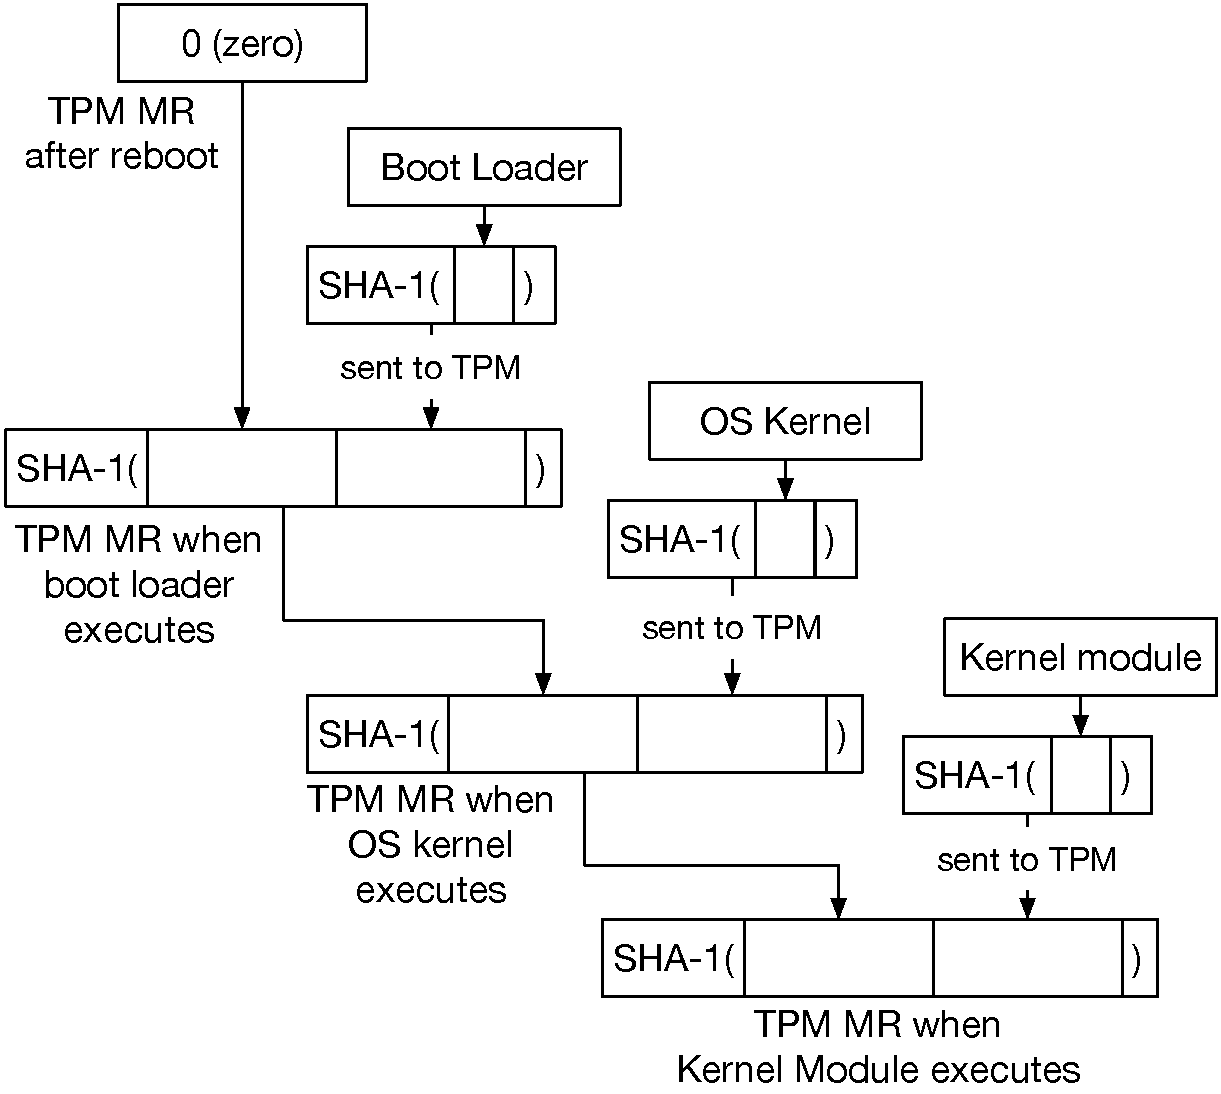
\includegraphics[width=85mm]{figures/tpm_measurement.pdf}
  \caption{
    The measurement stored in a TPM platform configuration register (PCR). The
    PCR is reset when the system reboots. The software at every boot stage
    hashes the next boot stage, and sends the hash to the TPM. The PCR's new
    value incorporates both the old PCR value, and the new software hash.
  }
  \label{fig:tpm_measurement}
\end{figure}

For example, the firmware on most modern computers implements the platform
initialization process in the Unified Extensible Firmware Interface (UEFI)
specification~\cite{forum2015uefi}. Each platform initialization phase is
responsible for verifying or measuring the firmware that implements the next
phase. The SEC firmware initializes the TPM PCR, and then stores the PEI's
measurement into a measurement register. In turn, the PEI implementation
measures the DXE firmware and updates the measurement register that stores the
PEI hash to account for the DXE hash. When the OS is booted, the hash in the
measurement register accounts for all the firmware that was used to boot the
computer.

Unfortunately, the security of the whole measurement scheme hinges on the
requirement that the first hash sent to the TPM must reflect the software that
runs in the first boot stage. The TPM threat model explicitly acknowledges this
issue, and assumes that the firmware responsible for loading the first stage
bootloader is securely embedded in the motherboard. However, virtually every
TPM-enabled computer stores its firmware in a flash memory chip that can be
re-programmed in software (\S~\ref{sec:motherboard}), so the TPM's measurement
can be subverted by an attacker who can reflash the computer's firmware
\cite{butterworth2013bios}.

On very recent Intel processors, the attack described above can be defeated by
having the initialization microcode (\S~\ref{sec:microcode_sec}) hash the
computer's firmware (specifically, the PEI code in UEFI \cite{forum2015uefi}
firwmare) and communicate the hash to the TPM chip. This is marketed as the
Measured Boot feature of Intel's Boot Guard \cite{ruan2014intelme}.

Sadly, most computer manufacturers use Verified Boot (also known as ``secure
boot'') instead of Measured Boot (also known as ``trusted boot''). Verified
Boot means that the processor's microcode only boots into PEI firmware that
contains a signature produced by a key burned into the chip's e-fuses. Verified
Boot does not impact the measurements stored on the TPM, so it does not improve
the security of software attestation.

\subsection{Intel's Trusted Execution Technology (TXT)}

Intel's Trusted Execution Technology (TXT) \cite{grawrock2009txt} uses the
TPM's software attestation model and auxilliary tamper-resistant chip, but
reduces the software inside the secure container to a virtual machine (guest
operating system and application) hosted by the CPU's hardware virtualization
features (VMX \cite{uhlig2005vmx}).

TXT isolates the software inside the container from untrusted software by
ensuring that the container has exclusive control over the entire computer
while it is active. This is accomplished by a secure initialization
authenticated code module (SINIT ACM) that effectively performs a warm system
reset before starting the container's VM.

TXT does not implement DRAM encryption or HMACs, and therefore is vulnerable to
physical DRAM attacks, just like TPM-based designs. Furthermore, early TXT
implementations were vulnerable to attacks where a malicious operating system
would program a device, such as a network card, to perform DMA transfers
to the DRAM region used by a TXT container \cite{wojtczuk2009txt,
wojtczuk2009txt2}. In recent Intel CPUs, the memory controller is integrated on
the CPU die, so the SINIT ACM
can securely set up the memory controller to reject DMA transfers targeting TXT
memory.

Early TXT implementations did not measure the SINIT ACM. Instead, the microcode
implementing the TXT launch instruction verified that the code module contained
an RSA signature by a hard-coded Intel key. SINIT ACM signatures cannot be
revoked if vulnerabilities are found, so TXT's software attestation had to be
revised when SINIT ACM exploits \cite{wojtczuk2011txt} surfaced. Currently, the
SINIT ACM's cryptographic hash is included in the attestation measurement.

Last, the warm reset performed by the SINIT ACM does not include the software
running in System Management Mode (SMM). SMM was designed
solely for the use of firmware, and is stored in a protected memory area
(SMRAM) which should not be accessible to non-SMM software. However, the SMM
handler was compromised on multiple occasions \cite{duflot2006smm,
rutkowska2008remap, wojtczuk2009smm, wecherowski2009smm, embleton2010smm}, and
an attacker that obtains SMM execution can access the memory used by TXT's
container.

\subsection{The Aegis Secure Processor}

The Aegis secure processor \cite{suh2003aegis} argued that Physically
Uncloneable Functions (PUFs) \cite{gassend2002puf} can be used to endow a
secure processor with a tamper-resistant private key, which is required for
software attestation. PUFs do not have the fabrication process drawbacks of
EEPROM, and are significantly more resilient to physical attacks than e-fuses.
Aegis relies on a security kernel in the operating system to isolate
containers, and includes the kernel's cryptographic hash in the measurement
reported by the software attestation signature.

Aegis relies on a trusted security kernel to isolate each container from the
other software on the computer by configuring the page tables used in address
translation. The security kernel is a subset of a typical OS kernel, and
handles virtual memory management, processes, and hardware exceptions. As the
security kernel is a part of the \textit{trusted code base} (TCB), its
cryptographic hash is included in the software attestation measurement. The
security kernel uses processor features to isolate itself from the untrusted
part of the operatings system, such as device drivers.

The Aegis memory controller encrypts the cache lines in one memory range, and
HMACs the cache lines in one other memory range. The two memory ranges can
overlap, and are configurable by the security kernel. Thanks to the two ranges,
the memory controller can avoid the latency overhead of cryptographic
operations for the DRAM outside containers. Aegis is not vulnerable to physical
replay attacks, as it uses a Merkle tree construction \cite{gassend2003merkle}
to guarantee DRAM freshness. The latency overhead of the Merkle tree is greatly
reduced by augmenting the L2 cache with the tree nodes for the cache lines.

Aegis' security kernel allows the OS to page out container memory, but verifies
the correctness of the paging operations. The security kernel uses the same
encryption and Merkle tree algorithms as the memory controller to guarantee the
privacy and integrity of the container pages that are swapped out from DRAM.
As the OS is free to page out container memory, it can learn a containter's
memory access patterns, at page granularity. Aegis containers are also
vulnerable to cache timing attacks.

\HeadingLevelB{The Bastion Architecture}
\label{sec:sgx_related_bastion}

The Bastion architecture \cite{champagne2010bastion} introduced the use of a
trusted hypervisor to provide secure containers to applications running inside
unmodified, untrusted operating systems. Bastion's hypervisor ensures that the
operating system does not interfere with the secure containers. We only
describe Bastion's virtualization extensions to architectures that use nested
page tables, like Intel's VMX \cite{uhlig2005vmx}.

The hypervisor enforces the containers' desired memory mappings in the OS page
tables, as follows. Each Bastion container has a Security Segment that lists
the virtual addresses and permissions of all the container's pages, and the
hypervisor maintains a Module State Table that stores an inverted page map,
associating each physical memory page to its container and virtual address. The
processor's hardware page walker is modified to invoke the hypervisor on every
TLB miss, before updating the TLB with the address translation result. The
hypervisor checks that the virtual address used by the translation matches the
expected virtual address associated with the physical address in the Module
State Table.

Bastion's cache lines are not tagged with container identifiers. Instead, only
TLB entries are tagged. The hypervisor's TLB miss handler sets the container
identifier for each TLB entry as it is created. Similarly to XOM and Aegis, the
secure processor checks the TLB tag against the current container's identifier
on every memory access.

Bastion offers the same protection against physical DRAM attacks as Aegis does,
without the restriction that a container's data must be stored inside a
continuous DRAM range. This is accomplished by extending cache lines and TLB
entries with flags that enable memory encryption and HMACing. The hypervisor's
TLB miss handler sets the flags on TLB entries, and the flags are propagated to
cache lines on memory writes.

The Bastion hypervisor allows the untrusted operating system to evict secure
container pages. The evicted pages are encrypted, HMACed, and covered by a
Merkle tree maintained by the hypervisor. Thus, the hypervisor ensures the
privacy, authenticity, and freshness of the swapped pages. However, the ability
to freely evict container pages allows a malicious OS to learn a container's
memory accesses with page granularity. Furthermore, Bastion's threat model
excludes cache timing attacks.

Bastion does not trust the platform's firmware, and computes the cryptographic
hash of the hypervisor after the firmware finishes playing its part in the
booting process. The hypervisor's hash is included in the measurement reported
by software attestation.

Intel's Software Guard Extensions (SGX)~\cite{mckeen2013sgx, anati2013sgx,
hoekstra2013sgx} implements secure containers for applications without making
any modifications to the processor's critical execution path. SGX does not
trust any layer in the computer's software stack (firmware, hypervisor, OS).
Instead, SGX's TCB consists of the CPU's microcode and a few privileged
containers. SGX introduces an approach to solving some of the issues raised by
multi-core processors with a shared, coherent last-level cache.

SGX does not extend caches or TLBs with container identity bits, and does not
require any security checks during normal memory accesses. As suggested in the
TrustZone documentation, SGX always ensures that a core's TLBs only contain
entries for the container that it is executing, which requires flushing the CPU
core's TLBs when context-switching between containers and untrusted software.

SGX follows Bastion's approach of having the untrusted OS manage the page
tables used by secure containers. The containers' security is preserved by a
TLB miss handler that relies on an inverted page map (the EPCM) to reject
address translations for memory that does not belong to the current container.

Like Bastion, SGX allows the untrusted operating system to evict secure
container pages, in a controlled fashion. After the OS initiates a container
page eviction, it must prove to the SGX implementation that it also switched
the container out of all cores that were executing its code, effectively
performing a very coarse-grained TLB shootdown.

SGX's microcode ensures the confidentiality, authenticity, and freshness of
each container's evicted pages, like Bastion's hypervisor. However, SGX relies
on a version-based Merkle tree, inspired by Aegis \cite{suh2003aegis}, and adds
an innovative twist that allows the operating system to dynamically shape the
Merkle tree. SGX also shares Bastion's and Aegis' vulnerability to memory
access pattern leaks, namely a malicious OS can directly learn a container's
memory accesses at page granularity, and any piece of software can perform
cache timing attacks.

SGX's software attestation is implemented using Intel's Enhanced Privacy ID
(EPID) group signature scheme \cite{brickell2009epid}, which is too complex for
a microcode implementation. Therefore, SGX relies on an assortment of
privileged containers that receive direct access to the SGX processor's
hardware keys. The privileged containers are signed using an Intel private key
whose corresponding public key is hard-coded into the SGX microcode, similarly
to TXT's SINIT ACM.

As SGX does not protect against cache timing attacks, the privileged enclave's
authors cannot use data-dependent memory accesses. For example, cache attacks
on the Quoting Enclave, which computes attestation signatures, would provide
an attack with a processor's EPID signing key and completely compromise SGX.

Intel's documentation states that SGX guarantees DRAM confidentiality,
authentication, and freshness by virtue of a Memory Encryption Engine (MEE).
The MEE is informally described in an ISCA 2015
tutorial~\cite{intel2015iscasgx}, and appears to lack a formal specification.
In the absence of further information, we assume that SGX provides the same
protection against physical DRAM attacks that Aegis and Bastion provide.

\HeadingLevelB{Sanctum}
\label{sec:related_sanctum}

Sanctum~\cite{costan2015sanctum} introduced a straightforward software/hardware
co-design that yields the same resilience against software attacks as SGX, and
adds protection against memory access pattern leaks, such as page fault
monitoring attacks and cache timing attacks.

Sanctum uses a conceptually simple cache partitioning scheme, where a
computer's DRAM is split into equally-sized continuous DRAM regions, and each
DRAM region uses distinct sets in the shared last-level cache (LLC). Each DRAM
region is allocated to exactly one container, so containers are isolated in
both DRAM and the LLC. Containers are isolated in the other caches by flushing
on context switches.

Like XOM, Aegis, and Bastion, Sanctum also considers the hypervisor, OS, and the
application software to conceptually belong to a separate container. Containers
are protected from the untrusted outside software by the same measures that
isolate containers from each other.

Sanctum relies on a trusted security monitor, which is the first piece of
firmware executed by the processor, and has the same security properties as
those of Aegis' security kernel. The monitor is measured by bootstrap code in
the processor's ROM, and its cryptographic hash is included in the software
attestation measurement. The monitor verifies the operating system's resource
allocation decisions. For example, it ensures that no DRAM region is ever
accessible to two different containers.

Each Sanctum container manages its own page tables mapping its DRAM regions,
and handles its own page faults. It follows that a malicious OS cannot learn the
virtual addresses that would cause a page fault in the container. Sanctum's
hardware modifications work in conjunction with the security monitor to make
sure that a container's page tables only reference memory inside the container's
DRAM regions.

The Sanctum design focuses completely on software attacks, and does not offer
protection from any physical attack. The authors expect Sanctum's hardware
modifications to be combined with the physical attack protections in Aegis or
Ascend.

\HeadingLevelB{Ascend and Phantom}

The Ascend \cite{fletcher2012ascend} and Phantom \cite{maas2013phantom} secure
processors introduced practical implementations of Oblivious RAM
\cite{goldreich1987oram} techniques in the CPU's memory controller. These
processors are resilient to attackers who can probe the DRAM address bus and
attempt to learn a container's private information from its DRAM memory access
pattern.

Implementing an ORAM scheme in a memory controller is largely orthogonal to the
other secure architectures described above. It follows, for example, that
Ascend's ORAM implementation can be combined with Aegis' memory encryption and
authentication, and with Sanctum's hardware extensions and security monitor,
yielding a secure processor that can withstand both software attacks and
physical DRAM attacks.

